% Chapter 2

\chapter{CMS Detector} % 

\label{Chapter 2} % For referencing the chapter elsewhere, use \ref{Chapter1} 

\lhead{Chapter 2. \emph{CMS Detector}} % This is for the header on each page - perhaps a shortened title

%----------------------------------------------------------------------------------------
The Compact Muon Solenoid (CMS\cite{CMSTDR}) is one of two general purpose detectors at the LHC which have performed exceptionally well during run 1. To allow the measurement of generic new physics the detector is required to meet high requirements. These include: good muon resolution over for $|\eta|<2.5$ and dimuon resolution of     $\approx 1\%$ at $100GeV/c^2$; good charged particle resolution in the inner tracker and ability to tag $\tau s$ and $b$ quarks; good electromagnetic energy resolution and efficient isolation of leptons and photons; hermetic hadronic calorimeters ($|\eta|<5$) with fine segmentation ($\Delta\eta\times\delta\phi<0.1\times0.1$) to allow the accurate determination of missing energy \cite{physreq}. The b-tagging and missing energy requirements are especially important in the case of the $\alpha_T$ SUSY search.

\begin{figure}
\centering
    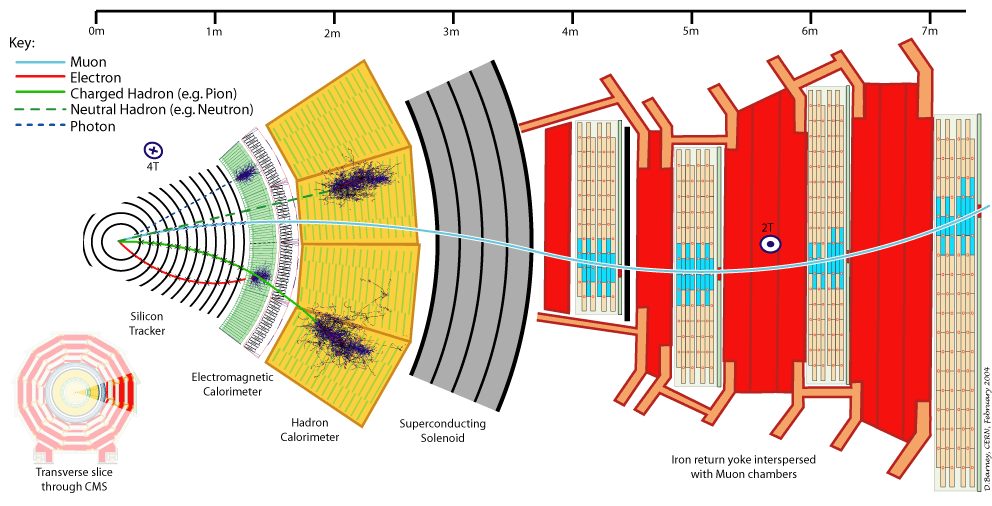
\includegraphics[width=0.9\textwidth]{./Figures/CMS_Slice.jpg}
  \caption{Cross Section of CMS showing the paths of various particle types through different segments of the detector \cite{cmsslice}}
  \label{CMS_SLICE}
\end{figure}

A cross section of CMS is shown in figure \ref{CMS_SLICE}. The coordinate system used by CMS takes the origin at the collision point. The z-axis points along the beam direction and defines the azimuthal angle, $\phi$. Instead of the polar angle, $\theta$, the psuedorapidity, $\eta=-ln(tan(\theta/2))$, is used as $\Delta \eta$ between two particles is relativistically invariant. The eta "coverage" of CMS is $|\eta|<5$. Transverse energies and momenta ($E_T $ and $p_T$)  are defined perpendicular to the beam \cite{cmsiop}. The different detector components shown in figure \ref{CMS_SLICE} will now be described in detail.
\begin{description}
\item[Silicon Tracker]The job of the tracker is to measure the momentum of charged particles from their path through a magnetic field. The CMS tracker achieves $10\mu m$ accuracy with coverage for $|\eta|<2.5$.
\item[Electromagnetic Calorimeter (ECAL)] The ECAL measures the energy of incident photons and electrons. The ECAL is made of 61,200 $PbWO_4$ crystals and provides coverage for $|\eta|<3.0$\cite{ecal}.
 \item[Hadronic Calorimeter (HCAL)] The HCAL is made from alternating brass and scintilator layers with a coverage of $|\eta|<3.0$\cite{hcal}. The coverage is extended to  $|\eta|<5.0$ by an iron/quartz forward calorimeter\cite{hfhcal}. 
 \item[Muon Chambers]The muons are not stopped by any of the calorimeters and therefore require a separate detector with coverage $|\eta| < 2.4$. The muon chambers are interspersed with the magnet return yoke. The high magnetic field allows for accurate momentum measurement\cite{muons}.
\end{description}